\documentclass[aspectratio=169]{beamer}
\usetheme{Madrid}
\usecolortheme{default}
\usepackage[utf8]{inputenc}
\usepackage[T5]{fontenc}
\usepackage{graphicx}
\usepackage{hyperref}
\usepackage{booktabs}
\usepackage{amsmath}
\usepackage{listings}
\usepackage{xcolor}

\definecolor{codegreen}{rgb}{0,0.6,0}
\definecolor{codegray}{rgb}{0.5,0.5,0.5}
\definecolor{codepurple}{rgb}{0.58,0,0.82}
\definecolor{backcolour}{rgb}{0.95,0.95,0.92}

\lstset{
    backgroundcolor=\color{backcolour},   
    commentstyle=\color{codegreen},
    keywordstyle=\color{magenta},
    numberstyle=\tiny\color{codegray},
    stringstyle=\color{codepurple},
    basicstyle=\ttfamily\scriptsize,
    breakatwhitespace=false,         
    breaklines=true,                 
    captionpos=b,                    
    keepspaces=true,                 
    numbers=left,                    
    numbersep=5pt,                  
    showspaces=false,                
    showstringspaces=false,
    showtabs=false,                  
    tabsize=2
}

\setbeamertemplate{caption}[numbered]
\renewcommand{\figurename}{Hình}
\renewcommand{\thefigure}{15.\arabic{figure}}

\title[Chương 15: Transformer]{Học Sâu (Deep Learning) \\ \vspace{0.5cm} \Large Chương 15: Mô hình Ngôn ngữ \& Kiến trúc Transformer}
\author{Đại học Đông Á}
\date{\today}

\begin{document}

\begin{frame}
    \titlepage
\end{frame}

\begin{frame}{Nội dung chương}
    \tableofcontents
\end{frame}

\section{1. Mô hình Ngôn ngữ \& Seq2Seq}

\begin{frame}{Language Model (Mô hình Ngôn ngữ) là gì?}
    \begin{itemize}
        \item Xuyên suốt khóa học, ta đã quen với việc phân loại (Classification). Nhưng để máy tính có thể "nói chuyện" và "tạo ra văn bản", ta cần một cách tiếp cận khác.
        \item \textbf{Language Model:} Một mô hình thống kê học phân phối xác suất: $P(\text{token\_tiếp\_theo} | \text{các\_token\_trước\_đó})$.
        \item Quá trình sinh văn bản (Text Generation): Dự đoán 1 token, ghép nó vào cuối chuỗi cũ, rồi lại đưa toàn bộ chuỗi mới vào mô hình để dự đoán token tiếp theo. Cứ lặp lại như vậy.
    \end{itemize}
\end{frame}

\begin{frame}[fragile]{Chuẩn bị dữ liệu Sinh văn bản: Văn thơ Shakespeare}
Để làm quen, ta sẽ dạy AI viết văn phong Shakespeare bằng cách đọc file text và cắt thành các chuỗi 100 ký tự.
\begin{lstlisting}[language=Python]
import keras
import tensorflow as tf

# Download Shakespeare dataset
filename = keras.utils.get_file(
    origin="https://storage.googleapis.com/download.tensorflow.org/data/shakespeare.txt"
)
shakespeare = open(filename, "r").read()

sequence_length = 100

def split_input(text, seq_len):
    for i in range(0, len(text), seq_len):
        yield text[i : i + seq_len]

# Features: text[:-1]. Labels: text[1:] (Shifted by 1 character)
features = list(split_input(shakespeare[:-1], sequence_length))
labels = list(split_input(shakespeare[1:], sequence_length))
dataset = tf.data.Dataset.from_tensor_slices((features, labels))
\end{lstlisting}
\end{frame}

\begin{frame}[fragile]{Xây dựng Bộ từ điển Cấp độ Ký tự (Char-level)}
\begin{lstlisting}[language=Python]
from keras import layers

# Map each character to an integer ID
tokenizer = layers.TextVectorization(
    standardize=None,
    split="character", # Split by char instead of word
    output_sequence_length=sequence_length,
)
tokenizer.adapt(dataset.map(lambda text, labels: text))

print(tokenizer.vocabulary_size()) # Output: 67 unique chars

dataset = dataset.map(
    lambda features, labels: (tokenizer(features), tokenizer(labels)),
    num_parallel_calls=8,
)
training_data = dataset.shuffle(10000).batch(64).cache()
\end{lstlisting}
\end{frame}

\begin{frame}[fragile]{Xây dựng Mô hình Ngôn ngữ Thu nhỏ (GRU)}
Mạng hồi quy \texttt{GRU} đọc chuỗi các ký tự và đưa ra xác suất 67 Class cho ký tự tiếp theo.
\begin{lstlisting}[language=Python]
embedding_dim = 256
hidden_dim = 1024

inputs = layers.Input(shape=(sequence_length,), dtype="int", name="token_ids")
x = layers.Embedding(tokenizer.vocabulary_size(), embedding_dim)(inputs)
x = layers.GRU(hidden_dim, return_sequences=True)(x)
x = layers.Dropout(0.1)(x)

# Output probabilities for the 67 characters in our vocab
outputs = layers.Dense(tokenizer.vocabulary_size(), activation="softmax")(x)
model = keras.Model(inputs, outputs)

model.compile(
    optimizer="adam",
    loss="sparse_categorical_crossentropy",
    metrics=["sparse_categorical_accuracy"],
)
model.fit(training_data, epochs=20)
\end{lstlisting}
\end{frame}

\begin{frame}[fragile]{Vòng lặp Sinh ký tự (Sampling Loop)}
Khác với Train, khi chạy thực tế (Inference), ta phải tạo một vòng lặp \textbf{Tự hồi quy} (Autoregressive): lấy output hiện tại đưa vào làm input cho bước tiếp theo.
\begin{lstlisting}[language=Python]
import numpy as np

generated_ids = []
max_length = 250

# Generate characters one by one
for i in range(max_length):
    # Predict probabilities for the next char
    predictions, state = generation_model.predict((inputs, state), verbose=0)
    
    # Pick the character with the highest probability
    next_char = int(np.argmax(predictions, axis=-1)[0])
    generated_ids.append(next_char)
    
    # The output becomes the new input
    inputs = keras.ops.expand_dims([next_char], axis=0)
\end{lstlisting}
\end{frame}

\begin{frame}{Kiến trúc Sequence-to-Sequence (Dịch máy)}
    \begin{columns}
        \column{0.5\textwidth}
        \begin{itemize}
            \item Sequence-to-Sequence (Seq2Seq) là bài toán biến một chuỗi đầu vào (Tiếng Anh) thành một chuỗi đầu ra (Tiếng Tây Ban Nha).
            \item Không thể dịch từng từ một (Word-by-word) vì ngữ pháp hai ngôn ngữ hoàn toàn khác nhau. Phải đọc trọn vẹn cả câu rồi mới bắt đầu dịch.
        \end{itemize}
        
        \column{0.5\textwidth}
        \begin{figure}
            \centering
            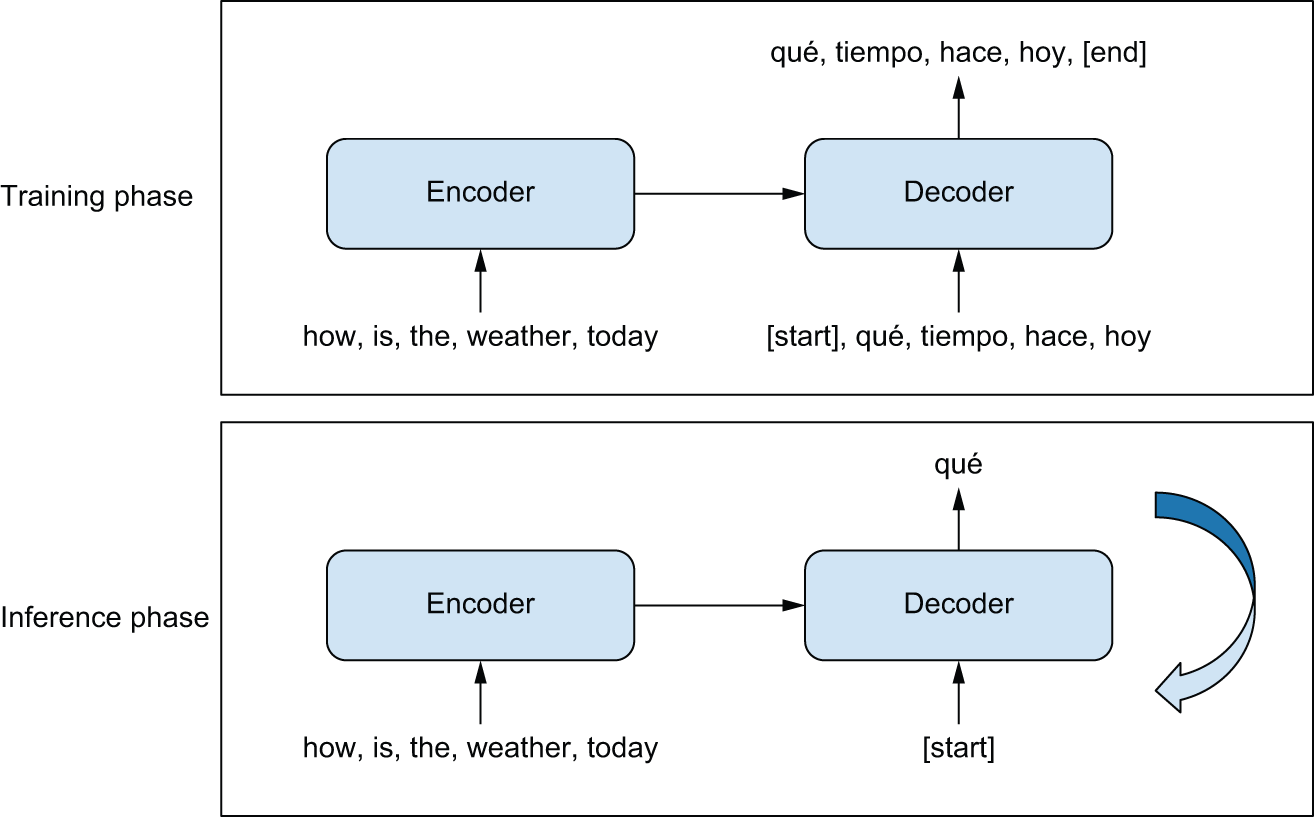
\includegraphics[width=\textwidth,height=0.6\textheight,keepaspectratio]{../../images/ch15/seq2seq-learning.0e1e1c31.png}
            \caption{Học chuỗi sang chuỗi (Seq2Seq)}
        \end{figure}
    \end{columns}
\end{frame}

\begin{frame}[fragile]{Chuẩn bị Dataset Đa đầu vào (Multi-Input Dataset)}
Bài toán Dịch máy yêu cầu dữ liệu rất đặc biệt. Bộ Giải mã (Decoder) cần biết \textbf{Câu nguồn tiếng Anh} và \textbf{Câu đích tiếng Tây Ban Nha bị dịch đi 1 từ}.
\begin{lstlisting}[language=Python]
def format_dataset(eng, spa):
    eng = english_tokenizer(eng)
    spa = spanish_tokenizer(spa)
    
    # Features contain BOTH the English source AND the Spanish input shifted
    features = {
        "english": eng, 
        "spanish": spa[:, :-1] # Drop the last token
    }
    
    # The targets are the Spanish sentence shifted forward
    labels = spa[:, 1:] # Drop the first token
    
    # Tell Keras to ignore padding tokens (0) when computing Loss
    sample_weights = labels != 0 
    
    return features, labels, sample_weights
\end{lstlisting}
\end{frame}

\begin{frame}{Nút thắt cổ chai của Seq2Seq sử dụng RNN/LSTM}
    \begin{columns}
        \column{0.5\textwidth}
        \begin{itemize}
            \item \textbf{Encoder (Bộ mã hóa):} Đọc toàn bộ câu Tiếng Anh, nén toàn bộ ý nghĩa vào một véc-tơ Trạng thái duy nhất (Context Vector).
            \item \textbf{Decoder (Bộ giải mã):} Lấy Context Vector đó làm điểm tựa để nhả ra từng từ Tiếng Tây Ban Nha.
            \item \textbf{Khuyết điểm chí mạng:} Context Vector trở thành nút thắt cổ chai (Bottleneck). Nếu câu văn quá dài (50 từ), một véc-tơ duy nhất không thể chứa nổi toàn bộ ngữ nghĩa.
        \end{itemize}
        
        \column{0.5\textwidth}
        \begin{figure}
            \centering
            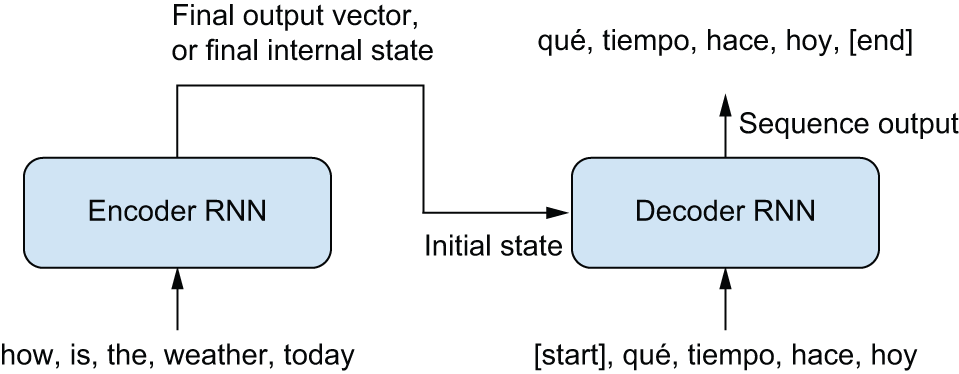
\includegraphics[width=\textwidth,height=0.6\textheight,keepaspectratio]{../../images/ch15/seq2seq-rnn.ec377d3b.png}
            \caption{Nút thắt của Seq2Seq RNN}
        \end{figure}
    \end{columns}
\end{frame}

\section{2. Cơ chế Chú ý (Attention Mechanism)}

\begin{frame}{Sự ra đời của Cơ chế Attention}
    \begin{columns}
        \column{0.5\textwidth}
        \begin{itemize}
            \item Tại sao phải nén toàn bộ câu vào 1 véc-tơ duy nhất? Tại sao không cho Decoder "nhìn" lại toàn bộ chuỗi đầu vào ở mỗi bước dịch?
            \item \textbf{Cơ chế Attention (2014):} Khi Decoder sinh ra từ thứ $t$, nó sẽ tự động tính toán xem trong số tất cả các từ của Encoder, từ nào là \textbf{quan trọng nhất} ở thời điểm hiện tại để "chú ý" vào.
        \end{itemize}
        
        \column{0.5\textwidth}
        \begin{figure}
            \centering
            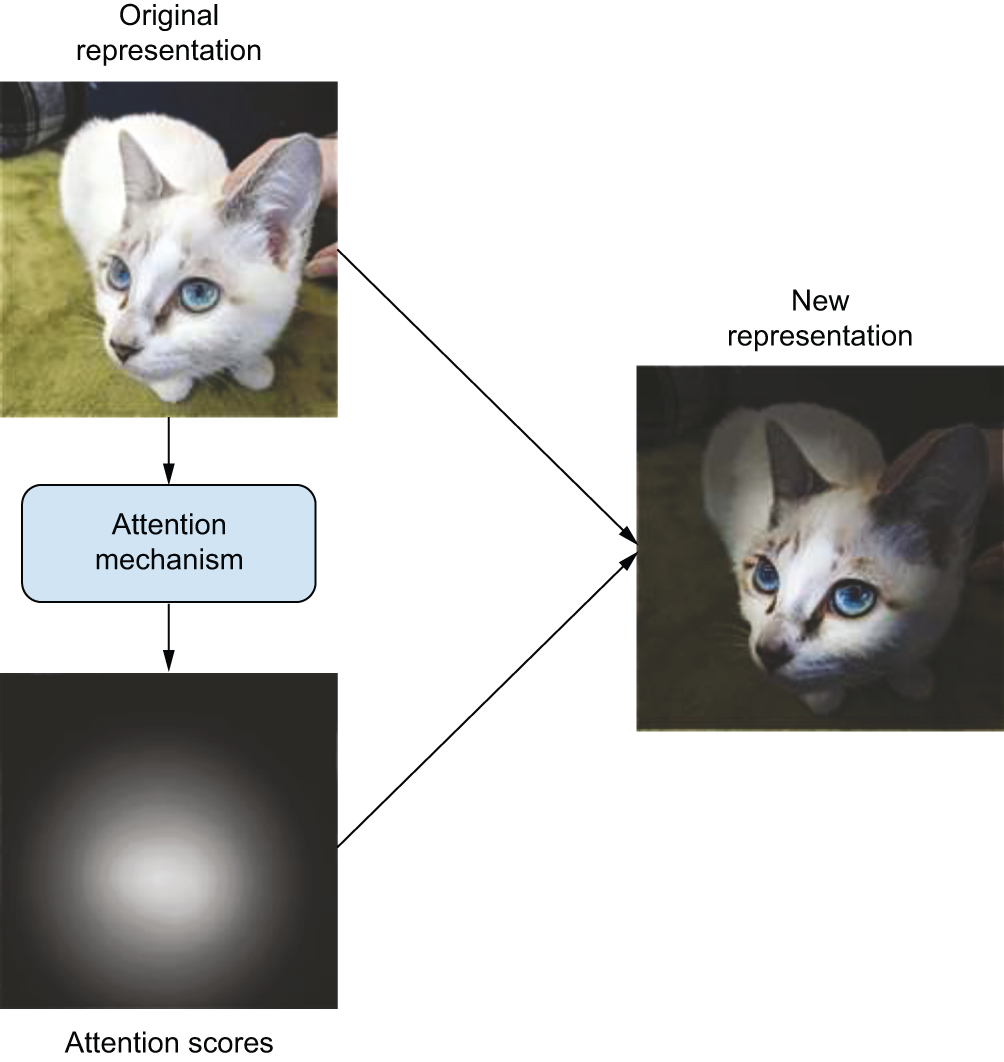
\includegraphics[width=\textwidth,height=0.6\textheight,keepaspectratio]{../../images/ch15/attention-concept.fde57742.png}
            \caption{Ý tưởng của Cơ chế Attention}
        \end{figure}
    \end{columns}
\end{frame}

\begin{frame}{Điểm Chú ý (Attention Scores)}
    \begin{columns}
        \column{0.5\textwidth}
        \begin{itemize}
            \item Điểm chú ý (Attention Scores) là tập hợp các trọng số từ $0$ đến $1$ (tổng bằng $1$).
            \item Ví dụ, khi Decoder đang dịch từ "station" (Trạm), nó sẽ gán điểm chú ý $0.95$ cho từ "estación" trong câu gốc, và gán gần $0.0$ cho các từ "I", "am", "at".
            \item Context Vector ở mỗi bước dịch giờ đây là Tích chập (Weighted Sum) của tất cả các trạng thái Encoder nhân với điểm chú ý.
        \end{itemize}
        
        \column{0.5\textwidth}
        \begin{figure}
            \centering
            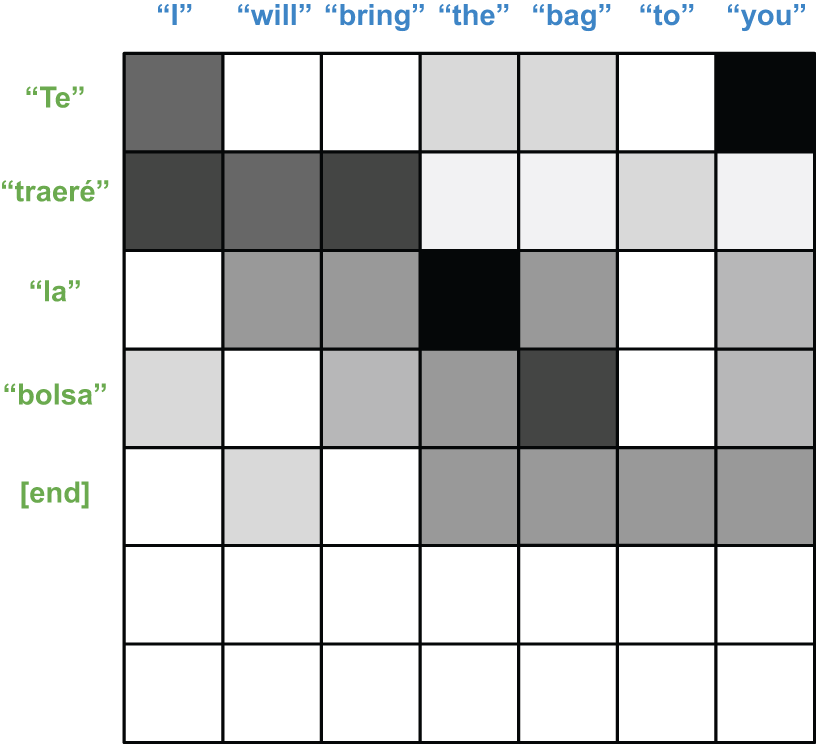
\includegraphics[width=\textwidth,height=0.6\textheight,keepaspectratio]{../../images/ch15/attention-scores.2932e0ff.png}
            \caption{Cách tính Toán học Attention Scores}
        \end{figure}
    \end{columns}
\end{frame}

\begin{frame}{Trực quan hóa Ma trận Attention}
    \begin{columns}
        \column{0.5\textwidth}
        \begin{itemize}
            \item Khi vẽ Ma trận điểm chú ý, ta thấy mô hình tự động học được cách "óng hàng" (Alignment) giữa 2 ngôn ngữ.
            \item Đặc biệt, nó xử lý hoàn hảo hiện tượng đảo ngữ pháp (VD: Tính từ đứng sau Danh từ trong tiếng Pháp/Tây Ban Nha).
        \end{itemize}
        
        \column{0.5\textwidth}
        \begin{figure}
            \centering
            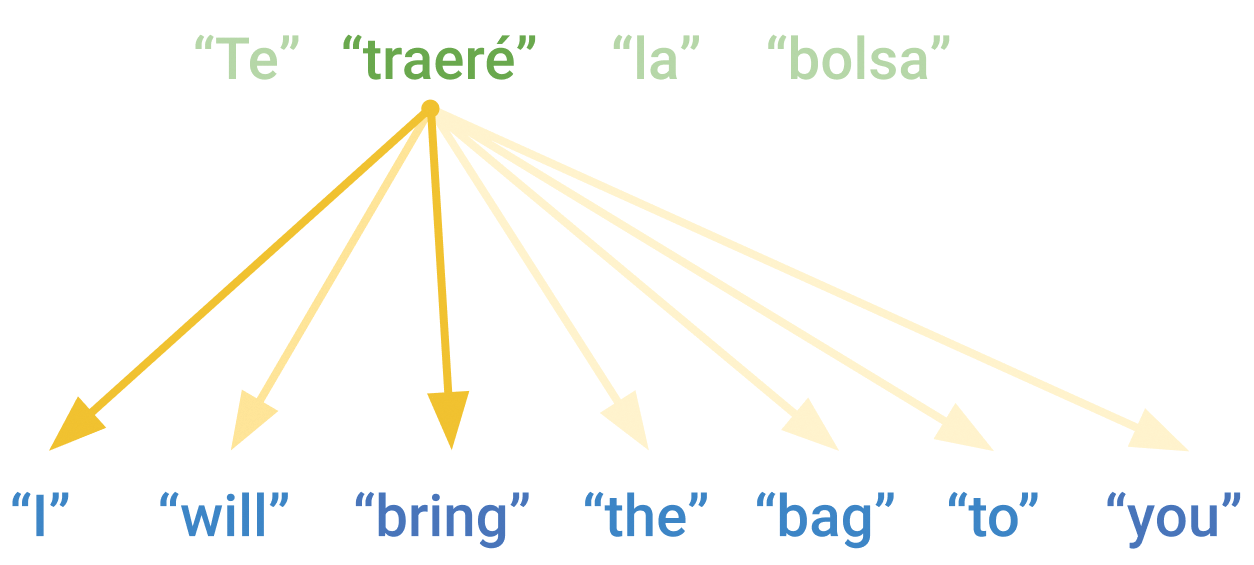
\includegraphics[width=\textwidth,height=0.6\textheight,keepaspectratio]{../../images/ch15/attention.6007731a.png}
            \caption{Biểu đồ phân bố Attention}
        \end{figure}
    \end{columns}
\end{frame}

\section{3. Self-Attention và Query-Key-Value}

\begin{frame}{Truy vấn Cơ sở dữ liệu: Query, Key, Value}
    \begin{columns}
        \column{0.5\textwidth}
        Để tổng quát hóa Attention, các nhà khoa học đã mượn khái niệm từ Hệ quản trị Cơ sở dữ liệu:
        \begin{itemize}
            \item \textbf{Query (Q):} Truy vấn ta đang tìm kiếm (Từ hiện tại đang xét).
            \item \textbf{Key (K):} Nhãn của các mục trong CSDL (Các từ khác trong câu).
            \item \textbf{Value (V):} Nội dung thực sự của các mục đó.
        \end{itemize}
        Mô hình sẽ so khớp $Q$ với tất cả các $K$. $K$ nào càng giống $Q$ thì $V$ của nó sẽ càng đóng góp nhiều vào kết quả.
        
        \column{0.5\textwidth}
        \begin{figure}
            \centering
            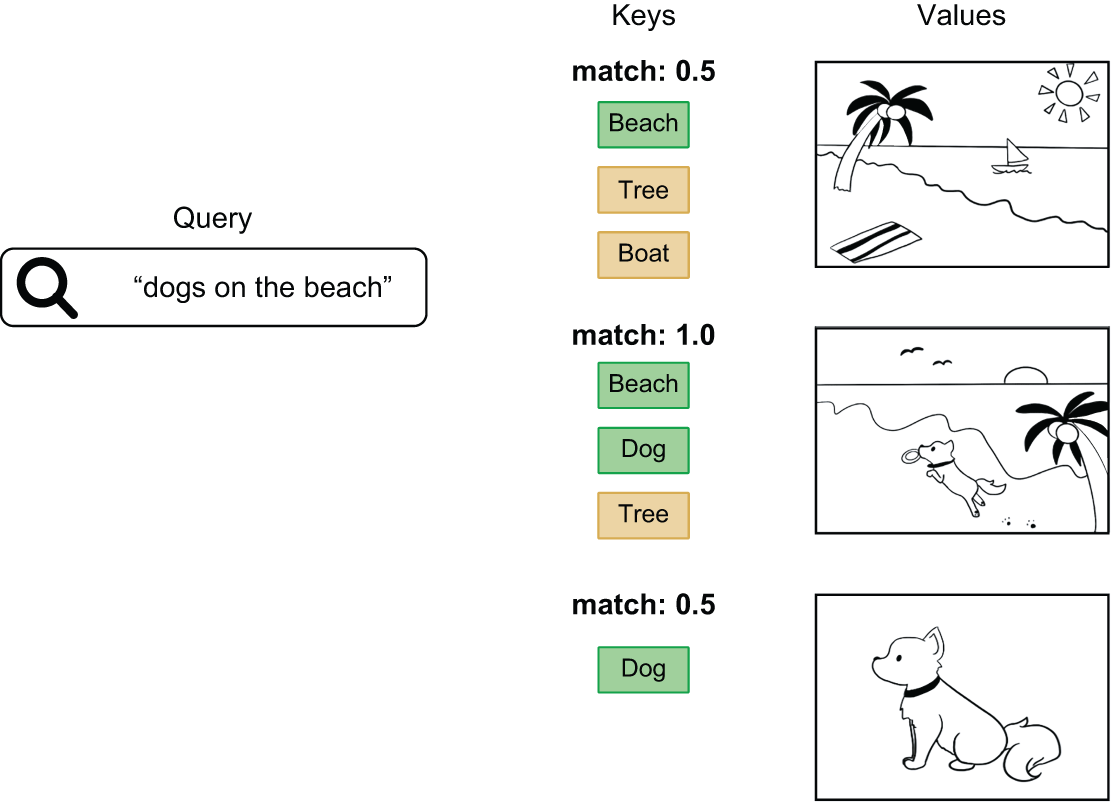
\includegraphics[width=\textwidth,height=0.6\textheight,keepaspectratio]{../../images/ch15/query-key-value.b57cceb0.png}
            \caption{Cơ chế Query - Key - Value}
        \end{figure}
    \end{columns}
\end{frame}

\begin{frame}{Phương trình Scaled Dot-Product Attention}
    \begin{itemize}
        \item Đây là phương trình Toán học quan trọng nhất thập kỷ của Trí tuệ Nhân tạo:
        $$ \text{Attention}(Q, K, V) = \text{softmax}\left(\frac{QK^T}{\sqrt{d_k}}\right)V $$
        \item \textbf{Giải thích:}
        \begin{itemize}
            \item $Q K^T$: Tích vô hướng (Dot Product) đo độ tương đồng giữa Query và toàn bộ Key.
            \item $\sqrt{d_k}$: Hệ số chia (Scaled) nhằm ổn định đạo hàm không bị quá lớn.
            \item $\text{softmax}$: Ép các điểm tương đồng thành xác suất phân bố từ $0$ đến $1$.
            \item $\times V$: Nhân kết quả xác suất với các Giá trị thực tế.
        \end{itemize}
    \end{itemize}
\end{frame}

\begin{frame}{Self-Attention (Tự Chú ý)}
    \begin{itemize}
        \item Điều gì xảy ra nếu $Q$, $K$, và $V$ đều đến từ \textbf{Cùng một chuỗi dữ liệu}?
        \item Đó gọi là \textbf{Self-Attention}. Nó cho phép một từ trong câu tự quan sát toàn bộ các từ còn lại trong chính câu đó để hiểu rõ ngữ cảnh của bản thân.
        \item Ví dụ câu: "The bank of the river" vs "The bank of America". Chữ "bank" sẽ tập trung sự chú ý vào "river" (bờ sông) hay "America" (ngân hàng) để thay đổi véc-tơ ngữ nghĩa của chính nó.
    \end{itemize}
\end{frame}

\begin{frame}{Multi-Head Attention (Chú ý Đa luồng)}
    \begin{columns}
        \column{0.5\textwidth}
        \begin{itemize}
            \item Thay vì chỉ tính Self-Attention 1 lần, ta tính nó $h$ lần song song (gọi là $h$ Heads).
            \item Tại sao? Vì một từ có rất nhiều khía cạnh: Ngữ pháp, Đại từ nhân xưng, Thời gian, Cảm xúc.
            \item Mỗi Head sẽ học cách "chú ý" vào một khía cạnh khác nhau của câu văn, làm cho không gian biểu diễn vô cùng phong phú.
        \end{itemize}
        
        \column{0.5\textwidth}
        \begin{figure}
            \centering
            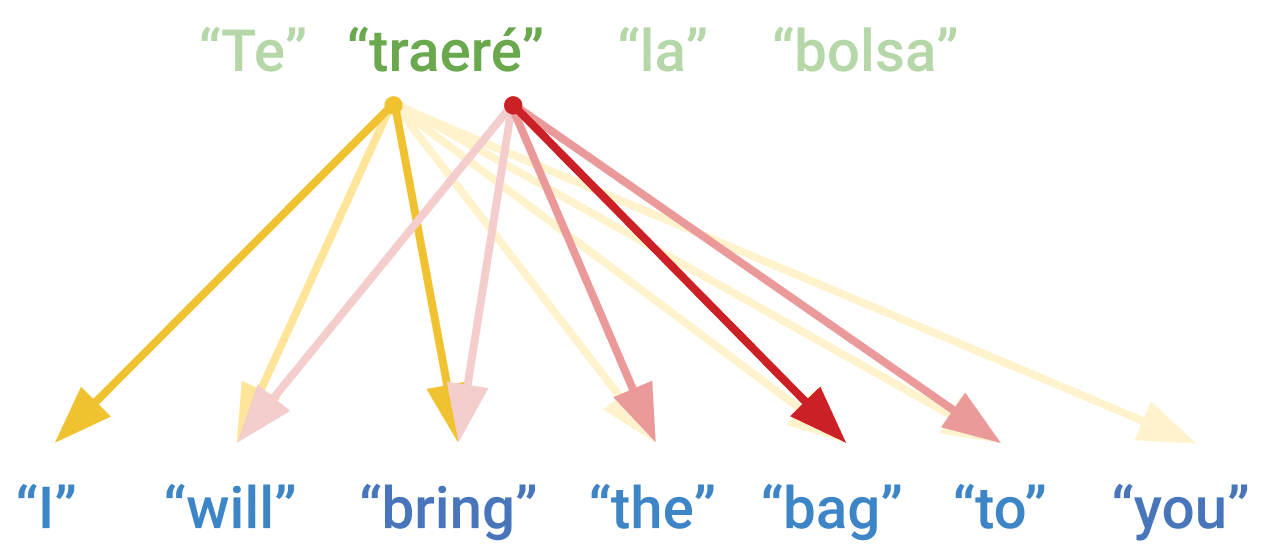
\includegraphics[width=\textwidth,height=0.6\textheight,keepaspectratio]{../../images/ch15/multi-head-attention.718456ad.png}
            \caption{Kiến trúc Multi-Head Attention}
        \end{figure}
    \end{columns}
\end{frame}

\begin{frame}[fragile]{Cài đặt khối Transformer Encoder}
Trong Transformer, không có LSTM. Chúng ta dựa hoàn toàn vào \texttt{MultiHeadAttention} và \texttt{Dense}. Kỹ thuật \textbf{Residual Connection} được dùng để tránh mất mát độ dốc.
\begin{lstlisting}[language=Python]
class TransformerEncoder(keras.Layer):
    def __init__(self, hidden_dim, intermediate_dim, num_heads):
        super().__init__()
        self.self_attention = layers.MultiHeadAttention(num_heads, hidden_dim // num_heads)
        self.self_attention_layernorm = layers.LayerNormalization()
        
        self.dense_1 = layers.Dense(intermediate_dim, activation="relu")
        self.dense_2 = layers.Dense(hidden_dim)
        self.dense_layernorm = layers.LayerNormalization()

    def call(self, source, source_mask):
        # 1. Self Attention with Residual Add & Norm
        residual = x = source
        x = self.self_attention(query=x, key=x, value=x, attention_mask=source_mask)
        x = self.self_attention_layernorm(x + residual)
        
        # 2. Feedforward with Residual Add & Norm
        residual = x
        x = self.dense_2(self.dense_1(x))
        return self.dense_layernorm(x + residual)
\end{lstlisting}
\end{frame}

\begin{frame}[fragile]{Sự khác biệt: Layer Normalization vs Batch Normalization}
Trong Transformer, chúng ta không dùng \texttt{BatchNormalization} (chuyên cho ảnh) mà dùng \texttt{LayerNormalization} (chuyên cho chuỗi).
\begin{lstlisting}[language=Python]
import numpy as np

# LayerNorm computes mean and variance for EACH sequence independently
def layer_normalization(batch_of_sequences):
    mean = np.mean(batch_of_sequences, keepdims=True, axis=-1)
    variance = np.var(batch_of_sequences, keepdims=True, axis=-1)
    return (batch_of_sequences - mean) / variance

# BatchNorm computes mean and variance ACROSS the entire batch
def batch_normalization(batch_of_images):
    mean = np.mean(batch_of_images, keepdims=True, axis=(0, 1, 2))
    variance = np.var(batch_of_images, keepdims=True, axis=(0, 1, 2))
    return (batch_of_images - mean) / variance
\end{lstlisting}
\end{frame}

\section{4. Kiến trúc Transformer}

\begin{frame}{Bài báo vĩ đại: "Attention Is All You Need" (2017)}
    \begin{itemize}
        \item Năm 2017, các nhà nghiên cứu Google tự hỏi: Nếu Attention mạnh mẽ như vậy, tại sao phải dùng RNN hay CNN nữa?
        \item Họ loại bỏ hoàn toàn RNN/CNN, chỉ thiết kế một mạng Nơ-ron cấu thành \textbf{hoàn toàn từ Multi-Head Attention}. Đó là \textbf{Transformer}.
        \item Ưu điểm tuyệt đối: Transformer có thể tính toán \textbf{Song song (Parallel)} trên GPU cho toàn bộ chuỗi cùng lúc, phá vỡ giới hạn tính tuần tự (từng từ một) chậm chạp của RNN.
    \end{itemize}
\end{frame}

\begin{frame}{Sơ đồ Kiến trúc Transformer}
    \begin{columns}
        \column{0.5\textwidth}
        \begin{itemize}
            \item Gồm 2 khối: Encoder (Bên trái) và Decoder (Bên phải).
            \item \textbf{Encoder:} Dùng Self-Attention để làm giàu ngữ cảnh cho câu đầu vào.
            \item \textbf{Decoder:} Dùng Causal Self-Attention (Che tương lai để không ăn gian) kết hợp với Cross-Attention (Lấy Q từ Decoder, K và V từ Encoder) để sinh từ tiếp theo.
        \end{itemize}
        
        \column{0.5\textwidth}
        \begin{figure}
            \centering
            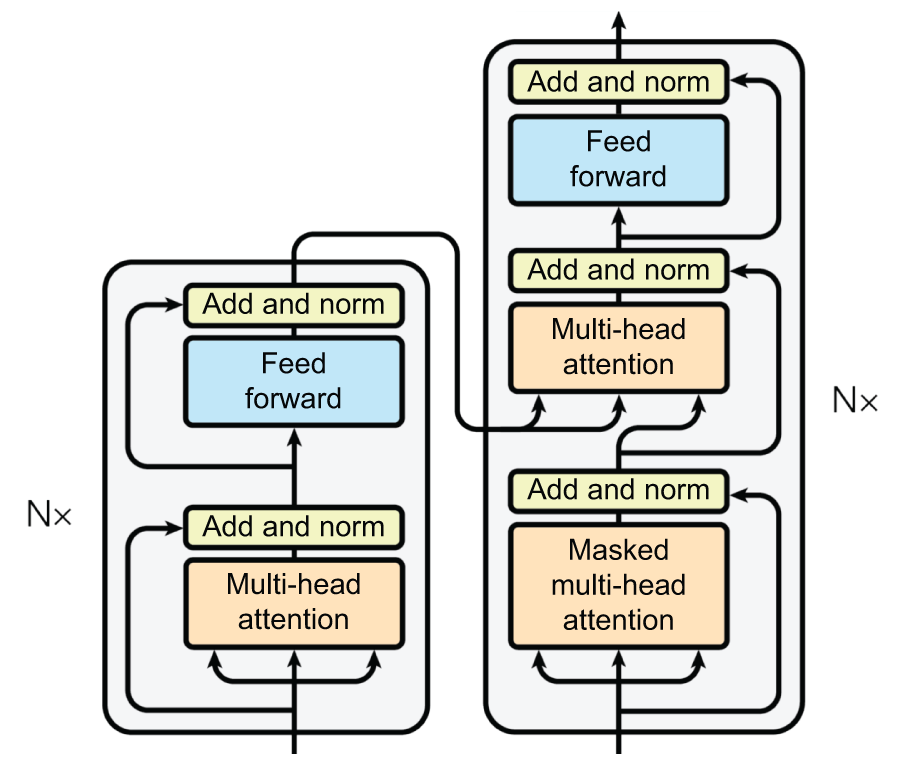
\includegraphics[width=\textwidth,height=0.6\textheight,keepaspectratio]{../../images/ch15/encoder-decoder.d979dbbc.png}
            \caption{Sơ đồ kinh điển của Transformer}
        \end{figure}
    \end{columns}
\end{frame}

\begin{frame}[fragile]{Cài đặt khối Transformer Decoder}
Decoder có tới 2 khối Attention. Khối đầu tiên là Causal Self-Attention. Khối thứ hai là Cross-Attention nhận Query từ Decoder và Key-Value từ Encoder.
\begin{lstlisting}[language=Python]
class TransformerDecoder(keras.Layer):
    def __init__(self, hidden_dim, intermediate_dim, num_heads):
        super().__init__()
        # Layers initialization omitted for brevity...

    def call(self, target, source, source_mask):
        # 1. Causal Self-Attention (Mask future words)
        residual = x = target
        x = self.self_attention(query=x, key=x, value=x, use_causal_mask=True)
        x = self.self_attention_layernorm(x + residual)
        
        # 2. Cross-Attention (Decoder attends to Encoder)
        residual = x
        x = self.cross_attention(query=x, key=source, value=source, attention_mask=source_mask)
        x = self.cross_attention_layernorm(x + residual)
        
        # 3. Feedforward 
        residual = x
        x = self.dense_2(self.dense_1(x))
        return self.dense_layernorm(x + residual)
\end{lstlisting}
\end{frame}

\begin{frame}[fragile]{Mặt nạ Causal Masking là gì?}
Trong \texttt{self\_attention} của Decoder, ta dùng tham số \texttt{use\_causal\_mask=True}. Điều này nhằm che đi các từ "tương lai". Nếu không có mặt nạ này, mô hình sẽ "ăn gian" nhìn thấy đáp án ngay trong dữ liệu luyện tập. Ma trận Causal trông như sau:
\begin{lstlisting}[language=Python]
[
    [1, 0, 0, 0, 0], # Token 0 only sees token 0
    [1, 1, 0, 0, 0], # Token 1 sees token 0, 1
    [1, 1, 1, 0, 0], # Token 2 sees token 0, 1, 2
    [1, 1, 1, 1, 0],
    [1, 1, 1, 1, 1],
]
\end{lstlisting}
Đây là cách Transformer giữ được tốc độ song song nhưng đảm bảo logic một chiều (như RNN).
\end{frame}

\begin{frame}{Mảnh ghép cuối: Positional Encoding (Mã hóa Vị trí)}
    \begin{itemize}
        \item Do tính toán song song, Transformer xử lý một câu giống như Bag-of-Words: Không hề biết từ nào đứng trước, từ nào đứng sau!
        \item Giải pháp: Cộng thêm một véc-tơ \textbf{Positional Encoding} (Dựa trên hàm Sine và Cosine hoặc Learnable Embeddings) vào véc-tơ Embedding của từ ban đầu.
        \item Nhờ đó, mỗi từ mang theo một "dấu vân tay" về vị trí của nó trong câu, giúp Transformer kết hợp tốc độ tính toán song song và khả năng hiểu ngữ pháp.
    \end{itemize}
\end{frame}

\begin{frame}[fragile]{Cài đặt Lớp Positional Embedding}
Tạo 2 Embedding: một cho Từ, một cho Vị trí (0, 1, 2...). Sau đó cộng chúng lại.
\begin{lstlisting}[language=Python]
from keras import ops

class PositionalEmbedding(keras.Layer):
    def __init__(self, sequence_length, input_dim, output_dim):
        super().__init__()
        self.token_embeddings = layers.Embedding(input_dim, output_dim)
        self.position_embeddings = layers.Embedding(sequence_length, output_dim)

    def call(self, inputs):
        # Generate position indices: [0, 1, 2, ..., sequence_length-1]
        positions = ops.cumsum(ops.ones_like(inputs), axis=-1) - 1
        
        # Get embeddings
        embedded_tokens = self.token_embeddings(inputs)
        embedded_positions = self.position_embeddings(positions)
        
        # Add them together
        return embedded_tokens + embedded_positions
\end{lstlisting}
\end{frame}

\begin{frame}[fragile]{Ráp nối Kiến trúc Transformer Hoàn chỉnh}
Gộp tất cả mọi thứ lại: Positional Embeddings $\rightarrow$ Encoder $\rightarrow$ Decoder $\rightarrow$ Dense.
\begin{lstlisting}[language=Python]
source = keras.Input(shape=(None,), dtype="int32", name="english")
x = PositionalEmbedding(sequence_length, vocab_size, hidden_dim)(source)
encoder_output = TransformerEncoder(hidden_dim, intermediate_dim, num_heads)(
    source=x, source_mask=source != 0
)

target = keras.Input(shape=(None,), dtype="int32", name="spanish")
x = PositionalEmbedding(sequence_length, vocab_size, hidden_dim)(target)
x = TransformerDecoder(hidden_dim, intermediate_dim, num_heads)(
    target=x, source=encoder_output, source_mask=source != 0
)

x = layers.Dropout(0.5)(x)
target_predictions = layers.Dense(vocab_size, activation="softmax")(x)

transformer = keras.Model([source, target], target_predictions)
transformer.compile(optimizer="adam", loss="sparse_categorical_crossentropy")
\end{lstlisting}
\end{frame}

\begin{frame}[fragile]{Kết quả Dịch máy Anh - Tây Ban Nha}
Sau khoảng 30 kỷ nguyên huấn luyện, Transformer đạt độ chính xác >67\% (Cao hơn rất nhiều so với mô hình RNN cùng kích thước).
\begin{lstlisting}[language=Python]
-
The resemblance between these two men is uncanny.
[start] el parecido entre estos cantantes de dos hombres son asombrosa [end]
-
I'll see you at the library tomorrow.
[start] te vere en la biblioteca manana [end]
-
Do you know how to ride a bicycle?
[start] sabes montar en bici [end]
\end{lstlisting}
\textit{Lưu ý: Mặc dù ngữ pháp có vài lỗi nhỏ, nhưng Transformer đã dịch chuẩn xác hầu hết các câu dài và ngữ cảnh phức tạp.}
\end{frame}

\begin{frame}{Tại sao Transformer lại vượt trội so với RNN?}
    \begin{itemize}
        \item \textbf{Hiệu suất song song (Parallelism):} RNN cần phải duyệt qua mã thông báo thứ $N-1$ mới có thể tính toán cho mã thông báo thứ $N$. Vòng lặp tuần tự này ngăn cản việc tận dụng sức mạnh tính toán song song của GPU.
        \item Transformer không có vòng lặp! Nó tính toán Attention cho \textbf{tất cả các mã thông báo cùng một lúc} thông qua phép nhân Ma trận. Điều này giúp tốc độ huấn luyện tăng lên gấp nhiều lần.
        \item \textbf{Ngữ cảnh tầm xa (Long-range context):} Trong RNN, thông tin ở đầu câu thường bị "quên" khi đến cuối câu. Với Self-Attention, mọi từ đều có kết nối trực tiếp $O(1)$ tới mọi từ khác trong câu, giải quyết hoàn hảo vấn đề giảm Gradient.
    \end{itemize}
\end{frame}

\begin{frame}{Mô hình Ngôn ngữ Che giấu (Masked Language Model)}
    \begin{itemize}
        \item Thay vì đoán từ tiếp theo như GPT, BERT (và RoBERTa) sử dụng \textbf{Masked Language Model (MLM)}.
        \item Thuật toán sẽ che ngẫu nhiên 15\% các từ trong câu bằng mã thông báo đặc biệt \texttt{[MASK]}. Sau đó, nó yêu cầu Transformer dùng các từ xung quanh để đoán xem từ bị che đi là gì.
        \item Ví dụ: "Con mèo đang ngủ trên chiếc \texttt{[MASK]} nhỏ." $\rightarrow$ Dự đoán: "giường".
        \item Nhờ cấu trúc Self-Attention hai chiều (Bidirectional), mô hình học được ngữ nghĩa của từ dựa trên toàn bộ các từ đứng trước và đứng sau nó.
    \end{itemize}
\end{frame}

\begin{frame}[fragile]{Kỷ nguyên của Pre-trained Transformers khổng lồ}
Mô hình Transformer dịch máy mà chúng ta vừa xây dựng có khoảng 14 triệu tham số. Các kiến trúc mạnh mẽ nhất trên thế giới hiện nay như BERT, RoBERTa hay GPT-4 có cấu trúc cốt lõi y hệt, nhưng được mở rộng lên tới \textbf{Hàng tỷ (Billions) tham số}.
\\ \vspace{0.3cm}
Bạn hoàn toàn có thể sử dụng sức mạnh này bằng \texttt{KerasHub}:
\begin{lstlisting}[language=Python]
import keras_hub

# Load the pretrained Tokenizer
tokenizer = keras_hub.models.Tokenizer.from_preset("roberta_base_en")

# Load the 124M parameter pretrained Transformer Backbone
backbone = keras_hub.models.Backbone.from_preset("roberta_base_en")

print(tokenizer("The quick brown fox"))
# Output: Array([133, 2119, 6219, 23602])
\end{lstlisting}
RoBERTa đã được "đọc" 160GB văn bản Tiếng Anh trên Wikipedia và Internet bằng hàng ngàn GPU. Nó tốn vài trăm ngàn Đô la chi phí tiền điện.
\end{frame}

\begin{frame}[fragile]{Tinh chỉnh (Fine-tuning) RoBERTa}
Ta có thể cắm thêm một lớp Dense vào đuôi của RoBERTa Backbone để dạy nó thực hiện mọi bài toán NLP mình muốn, từ Phân loại Cảm xúc đến Tìm kiếm thông tin. Quá trình này diễn ra cực kỳ nhanh và chuẩn xác.
\begin{lstlisting}[language=Python]
# Attach a Classification Head to RoBERTa
classifier = keras_hub.models.TextClassifier.from_preset(
    "roberta_base_en",
    num_classes=2,
)

classifier.compile(
    loss=keras.losses.SparseCategoricalCrossentropy(from_logits=True),
    optimizer="adam",
    metrics=["accuracy"],
)

# Fine-tune on our small IMDb Dataset
classifier.fit(train_ds, validation_data=val_ds, epochs=1)
\end{lstlisting}
\end{frame}

\section{Tổng kết}

\begin{frame}{Tổng kết Chương 15}
    \begin{itemize}
        \item \textbf{Sequence-to-Sequence:} Mô hình nền tảng cho Dịch máy, nhưng RNN vướng phải nút thắt cổ chai về véc-tơ ngữ cảnh.
        \item \textbf{Attention Mechanism:} Giải quyết bằng cách tính điểm trọng số cho toàn bộ câu đầu vào tại mỗi bước sinh từ.
        \item \textbf{Q-K-V Self-Attention:} Thuật toán tối thượng (Scaled Dot-Product) cho phép từ trong câu tự ánh xạ lên các từ khác để hiểu sâu ngữ cảnh.
        \item \textbf{Transformer:} Kiến trúc loại bỏ RNN, sử dụng hoàn toàn Multi-Head Attention. Đây chính là "trái kế" cấu thành nên các siêu AI như ChatGPT, GPT-4, BERT hiện nay.
    \end{itemize}
\end{frame}

\end{document}
